\chapter{Monitorowanie procesu gojenia ścięgna Achillesa}
\section{Ścięgno Achillesa}
Ścięgno Achillesa, nazywane również ścięgnem piętowym, jest największym i najsilniejszym ścięgnem występującym w ciele ludzkim. Stanowi wspólne zakończenie mięśnia trójgłowego łydki, w którego skład wchodzą dwie głowy mięśnia brzuchatego i mięsień płaszczkowaty. Całość struktury zlokalizowana jest w tylnym, powierzchownym przedziale łydki, co zostało przedstawione na Rysunku \ref{muscle_structure}.  
\begin{figure}[h!]
\centering
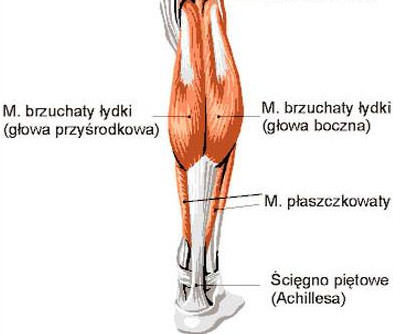
\includegraphics[width=0.55\textwidth]{figures/muscleStructure.jpg}
\caption{Lokalizacja mięśnia trójgłowego łydki wraz ze ścięgnem Achillesa.}
\label{muscle_structure}
\end{figure}
Z obu głów (brzuścców) mięśnia brzuchatego łydki wyrasta jedno szerokie, płaskie ścięgno, które jest początkiem części brzuchatej ścięgna Achillesa. Następnie ścięgno to łączy się z włóknami pochodzącymi od mięśnia płaszczkowatego, które układają się stycznie do wcześniej powstałej struktury. Wówczas kształt ulega stopniowemu zwężeniu i zaokrągleniu, aż do punktu o minimalnej szerokości (około 4 cm nad przyczepem dolnym [1]). W rejonie samego przyczepu dolnego znajdującego się na tylnej powierzchnia kości piętowej, ścięgno ponownie jest płaskie i szerokie.

W kolejnych podsekcjach szczegółowo omówiona została anatomia ścięgna Achillesa, jego biomechanika, potencjalne urazy wraz z czynnikami im sprzyjającymi oraz proces gojenia i możliwości jego wspomagania. Wszystkie te aspekty są istotne z uwagi na możliwości monitorowania procesów fizjologicznych występujących w ścięgnie. 
\subsection{Anatomia}
Średnia długość ścięgna Achillesa to 15 cm (11 - 26 cm). Średnia szerokość w rejonie początku wynosi 6.8 cm (4,5 - 8, 6 cm). Następnie, stopniowo ścięgno ulega zwężeniu do punktu o minimalnej szerokości 1.8 cm (1,2 - 2,6 cm). W rejonie samego przyczepu struktura ponownie się rozszerza i jej szerokość wynosi średnio 3.4 cm (2,0 - 4,8 cm) [2-3].
Zewnętrzną część ścięgna Achillesa stanowi ościęgno utworzone z tkanki łącznej włóknistej.
Achil
-Histologia
-Unaczynienie (krew, nerwy)

\subsection{Biomechanika}
Zadaniem ścięgien jest transfer siły mięśniowej do układu szkieletowego.
\subsection{Urazy i czynniki im sprzyjające}
\subsection{Leczenie, fazy gojenia i rehabilitacja}
\label{gojenie}
\section{Zastosowanie rezonansu magnetycznego}
Obrazowanie metodą \textit{Magnetycznego Rezonansu}, w skr. \textit{MR} (ang. \textit{Magnetic Resonance Imaging}, w skr. \textit{MRI}) jest metodą bazującą na odpowiednim odczycie reakcji atomów na silne pole magnetyczne. Zrozumienie tych procesów było efektem prac związanych z mechaniką kwantową takich jak: Einstein, Edwin Shrodinger, Heisenberg czy Pauli /*uzupełnij z licznych książek - krótką historię*/. Wymienione prace z początku XX wieku umożliwiły rozwój technologii MR zainicjowane zrozumieniem w latach 30-tych magnetycznej natury \textit{protonów}, cząstek subatomowych, które wraz z \textit{neutronami} wchodzą w skład jądra atomowego (zob. [1933 - stern gerlach]).

Dokładniej rzecz biorąc, główną własnością jądra atomowego umożliwiającą działanie MR jest \textit{spin}. Można powiedzieć, że jądro posiada spin jeżeli nie ma jednocześnie parzystej liczby protonów i parzystej liczby neutronów (por. [Rezonans magnetyczny]). Jądra o parzystej liczbie atomowej mają w \textit{stanie podstawowym} (charakteryzującym się najniższą energią) spin całkowity, a o nieparzystej połówkowy.

Cząstki o niezerowym spinie pochłaniają fale elektromagnetyczne o specyficznej częstotliwości konwertując energię na ruch rotacyjny nazywany \textit{rezonansem magnetycznym}. Zjawisko to opisuje się równaniem Larmora \ref{MRLarmor}:
\begin{equation}
\label{MRLarmor}
\omega_0 = \gamma \ast \beta_0,
\end{equation}
gdzie $\omega_0$ to prędkość obrotowa protonów (tzw. częstotliwość Larmora), $\gamma$ to współczynnik żyromagnetyczny właściwy danemu protonowi, a $\beta_0$ to wartość zadanego pola magnetycznego. Dla przykładu częstotliwość Larmora dla protonu wodoru, gdzie $\gamma$=42,57 MHz/T dla pola 1,5T równa jest 63,8 MHz. Wodór jest najczęściej wykorzystywanym pierwiastkiem w metodzie rezonansu magnetycznego, gdyż jest obecny w 99,98\% ludzkich tkanek (za [MR]). Jednak w szczególnych przypadkach stosuje się również obrazowania z wykorzystaniem częstotliwości odpowiednich dla fosforu, sodu czy węgla (zob. []).

Rezonujące protony mają własności podobne do magnesów prętowych i mogą być ukierunkowane przy pomocy pola magnetycznego. Protony o wysokich poziomach energii odchylają się przeciwnie do kierunku zadanego pola magnetycznego tzw. \textit{protony antyrównoległe}, a o niskich poziomach energii odchylają się zgodnie z kierunkiem pola tzw. \textit{protony równoległe}. W przeciętnym wycinku ciała ludzkiego jest więcej protonów równoległych niż antyrównoległych. Przykładowo w objętości 1 $\times$ 1 $\times$ 5 mm jest to liczba około 2 $\times$ $10^15$ cząstek.

Z uwagi na różne parametry mierzone w reakcji protonów na zadane pole magnetyczne powstało wiele różnych sekwencji MR, które mają często odmienne własności aplikacyjne. W tej pracy zostało użytych 10 różnych sekwencji MR. Zostaną one pokrótce scharakteryzowane w kolejnych punktach:
\begin{itemize}
	\item \textit{T1} -- mierzona jest \textit{relaksacja T1}, a zatem czas potrzebny protonom na powrót do stanu początkowego po odchyleniu o 90$^\circ$. Sygnał rezonansu magnetycznego $MR_s$ można obliczyć z zależności:
	\begin{equation}
		MR_s \sim \gamma_{pd} \ast [1-e^{-TR/T1}],
	\end{equation}
	gdzie $\gamma_{pd}$ to gęstość protonowa tkanki, $TR$ to \textit{czas repetycji} określany przez użytkownika.
	\item \textit{T2} -- mierzona jest \textit{relaksacja T2}, tj. czas potrzebny do utraty spoistości pomiędzy między spinami. Dokładniej mówiąc różnice w częstotliwości Larmora powstające w czasie, wynikające z umiejscowienia protonów w różnych ośrodkach i niejednorodności w pobudzeniach polem magnetycznym. $MR_s$ przyjmuje wówczas następującą zależność:
	\begin{equation}
	MR_s \sim \gamma_{pd} \ast [1-e^{-TE/T2}],
	\end{equation}
	gdzie $TE$ to \textit{czas echa} zdefiniowany przez użytkownika.
	\item \textit{PD} (od ang. \textit{Proton Density}) -- mierzona jest gęstość spinowa tkanki wprost proporcjonalna do liczby protonów. Wówczas:
	\begin{equation}
	MR_s \sim \gamma_{pd}.
	\end{equation}
	\item \textit{T2 mapping} -- dla wielu TE
	\item \textit{T2 $^\ast$ GRE} (od ang. \textit{Gradient Echo}) -- w sekwencjach gradientowych protony odchylane są o kąt mniejszy od $90^\circ$ (zazwyczaj 10$^\circ$ -- 80$^\circ$). $MR_s$ jest wówczas zależne od obu czynników $T1$ i $T2$:
	\begin{equation}
	MR_s \sim \gamma_{pd} \ast [1-e^{-TE/T2}][1-e^{-TR/T1}],
	\end{equation}
	przy czym dla mniejszych kątów wkład $T2$ rośnie w stosunku do wkładu $T1$.
	\item \textit{T2 $^\ast$ GRE TE\_MIN} (od ang. \textit{Minimal Time Echo}) --
	\item \textit{3D FSPGR In Phase Ideal} (od ang. \textit{Fast Spoiled Gradient Echo}) -- spoiled to rozfazowanie
	\item \textit{3D FSPGR Out Phase Ideal} --
	\item \textit{3D FSPGR Fat Ideal} --
	\item \textit{3D FSPGR Water Ideal} -- 
\end{itemize}

/*akapit o tworzeniu obrazu*/



/* chyba jednak do USG - fala, amplituda, częstotliwość*/ 
\section{Zastosowanie ultrasonografii}

Kolejną z metod obrazowania medycznego jest \textit{Ultrasonografia}, w skr. \textit{USG} (ang. \textit{Ultrasonography}, \textit{US}). Bazuje ona na efektach związanych z propagacją w tkankach \textit{ultradźwięków}, tj. fal akustycznych o częstotliwościach powyżej 20 kHz.

Propagacja fal w przyrodzie była tematem rozważań myślicieli takich jak Pitagoras, Arystoteles czy Galileusz, którzy ugruntowali pole badań pod kolejne osiągnięcia matematyczno-inżynieryjne. W tej kwestii, do jednego z przełomów doszło w 1822 roku, kiedy to szwajcarski inżynier Daniel Colladen oraz matematyk Charles-Francois Sturm wyznaczyli przybliżoną prędkość rozchodzenia się fali akustycznej w wodzie. Badanie wykonano na Jeziorze Genewskim symultanicznie mierząc czas jaki potrzebny był dźwiękowi podwodnego wystrzału i sygnałowi dzwonka rozchodzącego się w powietrzu do przebycia drogi pomiędzy dwoma łódkami oddalonymi o 10 mil. Wyliczona wartość wyniosła wówczas 1435 m/s nie różniąc się znacząco od dzisiaj przyjmowanej estymacji równej 1480 m/s. Analogicznie wyliczane są obecnie prędkości rozchodzenia się w fali w innych ośrodkach takich jak powietrze, tkanki miękkie, kości itp.

58 lat później, w 1880 roku bracia Curie opisali w \cite{Curie1880} \textit{efekt piezoelektryczny}, czyli zjawisko polegające na pojawieniu się ładunku elektrycznego pod wpływem naprężeń mechanicznych w krysztale o anizotropowej budowie, takiej jak ma np. kwarc. W przypadku odwrotnym, przyłożenie napięcia do odpowiedniego kryształu generuje drgania. 

Efekty te są wykorzystywane w \textit{głowicy aparatu usg}, przyrządu do generowania i odbierania ultradźwięków. Przykładowo, polaryzowanie kryształu piezoelektrycznego krótkim impulsem elektrycznym $\sigma_1(t)$ pobudza go do drgań na własnej częstotliwości rezonansowej. Zakładając, że kryształ ma kształt walca o grubości $d$=0,64mm, to będzie stanowił rezonator półfalowy, w którym wystąpi drganie rezonansowe o długości fali $\lambda = 2d$ czyli $\lambda = 1,28$ mm. Jeżeli wykonany jest z tytanianu baru, dla którego prędkość propagacji drgań wynosi $c$=4460m/s, to częstotliwość drgań własnych tego
kryształu wyniesie:
\begin{equation}
f = \frac{c}{\lambda} = \frac{4460 m/s}{1,28 mm} = 3,5 MHz.
\end{equation}
Odwrotnie, powracająca fala tzw. \textit{echo} wygeneruje impuls elektryczny $\sigma_2(t)$ w skutek drgań wywołanych w krysztale. 
 
Echo jest naturalnie falą różniącą się od sygnału nadawanego, a zmiany te są w przeważającym stopniu efektem zjawisk znanych z optyki falowej tj. \textit{odbicia}, \textit{załamania}, \textit{dyfrakcja}, \textit{rozpraszanie} i \textit{pochłanianie} (zob. []).

Zależą one on częstotliwości fali, która propaguje się w ośrodku o pewnej \textit{impedancji akustycznej ośrodka} $Z$ wyrażanej jako:
\begin{equation}
Z = \rho c = \sqrt{\epsilon \rho},
\end{equation}
gdzie $c$, to prędkość rozchodzenia się fali, $\rho$ to gęstość ośrodka, a $\epsilon$ to \textit{moduł odkształcalności objętościowej}, tj. parametr opisujący jak zmieni się objętość ośrodka pod danym ciśnieniem. Parametry wybranych ośrodków zestawiono w Tabeli \ref{USG-params} 
\begin{figure}[h!]
	\centering
	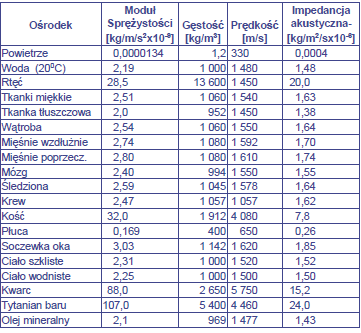
\includegraphics[width=0.55\textwidth]{figures/USG-params.png}
	\caption{Parametry ośrodków często mierzonych w badaniach USG.}
	\label{USG-params}
\end{figure}

Dla przykładu, do zjawiska załamania lub odbicia dochodzi kiedy fala pada na granice dwóch ośrodków o różnych impedancjach akustycznych $Z_1$ i $Z_2$. Zależność ta opisana jest prawem Snella:
\begin{equation}
R = \frac{I_r}{I_0} = \left(\frac{Z_1-Z_2}{Z_1+Z_2}\right)^2,
\end{equation}
gdzie $I_r$ to natężenie fali padającej, a $I_0$ odbitej. Natomiast $R$, czyli współczynnik odbicia, jest parametrem, który rośnie wraz ze wzrostem kąta odchylenia od kierunku prostopadłego, aż do całkowitego odbicia.

Z kolei do rozpraszania bądz pochłaniania fali dochodzi kiedy to fala pokonuje daną drogę w ośrodku o pewnej $Z$, co zapisywane jest następująco:
\begin{equation}
I=I_0 \epsilon^{-\gamma x},
\end{equation}
gdzie $\gamma$ to współczynnik osłabienia zależny od $Z$, a $x$ to droga przebyta przez falę. Efekt ten można korygować poprzez dobór odpowiedniego $I_0$.

Analiza amplitudy i częstotliwości sygnału nadanego i echa umożliwia rekonstrukcję obrazu USG. W przypadku najczęściej stosowanych w praktyce rekonstrukcji przekrojów dwuwymiarowych (tzw. tryb B) współczesny tor budowania prezentacji wizualnej (tzw. \textit{beamforming}) wygląda następująco: 
\begin{enumerate}
	\item Głowica ultradźwiękowa emituje impulsy w postaci wąskiej wiązki w ściśle określonym kierunku. Wiązka zawiera sygnał z $N$ przetworników zawierających kryształy piezoelektryczne.
	\item Echa z danego kierunku pozwalają na obliczenie pojedynczego promienia akustycznego, który jest iloczynem charakterystyk nadawanego i odbieranego sygnału.
	\item Wszystkie promienie, których we współczesnych aparatach może być do kilkuset (zob. [GE Voluson]), służą do formowania obrazu, który tworzony jest we \textit{współrzędnych biegunowych} ($r$, $\theta$) w przypadku głowic mechanicznych sektorowych, wieloelementowych convex czy fazowych lub we współrzędnych prostokątnych ($x$, $y$) w przypadku głowic mechanicznych lub wieloelementowych liniowych\footnote{szczegółowy opis głowic USG i ich charakterystyk można znalezć w []}. 
\end{enumerate}

Tryb B umożliwia również wizualizację obrazów dynamicznych. Przykładowo jeżeli na obraz składa się 400 promieni i każdy odsłuchiwany jest do głębokości 15cm, to czas gromadzenia danych dla ośrodka o średnim c=1500 m/s wynosi $2\frac{2\times15}{1500 m/s}\times400 = 0,08 s$, czyli 12 obrazów na sekundę. Częstotliwość tę można zwiększać, zmniejszając liczbę promieni lub głębokość obserwacji.

Innym często stosowanym trybem rekonstrukcji obrazu (wykorzystywanym również w tej pracy) jest tryb D bazujący na \textit{efekcie Dopplera}, do którego dochodzi w przypadku przechodzenia fali przez ośrodki względem siebie się przesuwające. Zmienia się wówczas częstotliwość fali, co wyrażone jest następującym wzorem:
\begin{equation}
f_r = 2 f_o\frac{v}{c}\cos(\theta),
\end{equation} 
gdzie $f_r$ to zmiana częstotliwości fali nadawanej $f_0$, zależna od kąta $\theta$ pomiędzy falą i ośrodkiem poruszającym się i prędkościami rozchodzenia się fali w obu ośrodkach tj. $v$ i $c$. Tryb D jest wykorzystywany w praktyce np. do monitorowania przepływu krwi w tkankach. 

W kontekście ścięgna Achillesa tryb B jest użyteczny do obrazowania tkanek miękkich. Przydatna jest zwłaszcza możliwość zobrazowania ukierunkowania struktur włókien ścięgnistych na podstawie czego radiolog może wnioskować o fazie gojenia. Składowa czasowa jest interesująca z perspektywy fizjoterapeuty oceniającego m.in. ślizg w ścięgnie przy wykonywaniu odpowiednich ruchów np. zginania podeszwowo-grzbietowego stopy. Tryb D natomiast może służyć do oceny unaczynienia ścięgna w kolejnych etapach gojenia, które jak wiadomo z sekcji \ref{gojenie} zmienia się w czasie.

W porównaniu do rezonansu magnetycznego USG charakteryzuje się niskimi kosztami aparatury. Uzyskiwane obrazy są jednak trudniejsze w interpretacji, co przekłada się na koszty wyszkolenia kadry. W tym kontekście przydatne mogą okazać się nowe rozwiązania w warstwie sprzętowej i oprogramowania. 

Do pierwszej grupy należy zaliczyć zastąpienie przetworników z piezoelektrykami, przetwornikami budowanymi w technologi MEMS np. cMUT, czy pMUT (zob. [butterfly-http://news.mit.edu/2018/startup-butterfly-network-ultrasound-smartphone-0207]) oraz układy pozwalające przetwarzać surowy sygnał ultradxwiękowy (zob. [us4us]). Do drugiej grupy należą algorytmy sztucznej inteligencji pozwalające wydobyć i zinterpretować interesującą informację z niskiej jakości obrazów (np. zob. [nvidia-keynot-clarisa-project]). 

Badania obrazowe nie są jedynymi, które służą do oceny gojenia się ścięgna Achillesa. W kolejnej sekcji zostały opisane metody oceny biomechaniki, które samodzielnie jak i w połączeniu z analizą obrazową stanowią wartościową informację diagnostyczną.

\section{Zastosowanie badań biomechanicznych}
\section{Inne metody}